\documentclass{article}[a4paper, oneside, 11pt]
\usepackage[T1]{fontenc}
\usepackage[utf8]{inputenc}
\usepackage{calc}
\usepackage{amsmath,amssymb,amsthm, thmtools, amsfonts}
\usepackage[nochapters,pdfspacing]{classicthesis}
%\usepackage{hyperref}% clashes with classicthesis
\usepackage{cleveref}
\usepackage[siunitx]{circuitikz}
\usepackage{booktabs}
\usepackage{graphicx}
\usepackage{caption}
\usepackage{geometry}
\usepackage{float}
\usepackage{mdframed}
\usepackage{xcolor}
\usepackage{siunitx}
\usepackage[italian]{babel}
\usepackage{pgfplots}
\usepackage{titling}
\usepackage{listings}
\usepackage{lmodern}
\usepackage{url}
\usepgfplotslibrary{external} 
\tikzexternalize

\pgfplotsset{compat=1.16}
\lstset{
basicstyle=\ttfamily,
columns=fullflexible,
keepspaces=true,
}
\mdfsetup{linewidth=0.6pt}
\graphicspath{{./figs/}}
\makeatletter
\def\input@path{{./figs/}}
%or: \def\input@path{{/path/to/folder/}{/path/to/other/folder/}}
\makeatother

\newcommand{\eps}{\varepsilon}
\renewcommand{\phi}{\varphi}
\newcommand{\loc}{\mathit{loc}}
\newcommand{\weakto}{\rightharpoonup}
\newcommand{\implied}{\Longleftarrow}
\let\subsetstrict\subset
\renewcommand{\subset}{\subseteq}
\renewcommand{\supset}{\supseteq}

% calligraphic letters
\newcommand{\A}{\mathcal A}
\newcommand{\B}{\mathcal B}
\newcommand{\C}{\mathcal C}
\newcommand{\D}{\mathcal D}
\newcommand{\E}{\mathcal E}
\newcommand{\F}{\mathcal F}
\newcommand{\FL}{\mathcal F\!\mathcal L}
\renewcommand{\H}{\mathcal H}
\newcommand{\K}{\mathcal K}
\renewcommand{\L}{\mathcal L}
\newcommand{\M}{\mathcal M}
\renewcommand{\P}{\mathcal P}
\renewcommand{\S}{\mathcal S}
\newcommand{\U}{\mathcal U} %% intorni

% blackboard letters
\newcommand{\CC}{\mathbb C}
\newcommand{\HH}{\mathbb H}
\newcommand{\KK}{\mathbb K}
\newcommand{\NN}{\mathbb N}
\newcommand{\QQ}{\mathbb Q}
\newcommand{\RR}{\mathbb R}
\newcommand{\TT}{\mathbb T}
\newcommand{\ZZ}{\mathbb Z}

%\newcommand{\abs}[1]{{\left|#1\right|}}
\newcommand{\Abs}[1]{{\left\Vert #1\right\Vert}}
\newcommand{\enclose}[1]{{\left( #1 \right)}}
\newcommand{\Enclose}[1]{{\left[ #1 \right]}}
\newcommand{\floor}[1]{\left\lfloor #1 \right\rfloor}
\newcommand{\ceil}[1]{\left\lceil #1 \right\rceil}

\newcommand{\To}{\rightrightarrows}
\renewcommand{\vec}[1]{\boldsymbol #1}
\newcommand{\defeq}{:=}
\DeclareMathOperator{\divergence}{div}
\renewcommand{\div}{\divergence}
\DeclareMathOperator{\Imaginarypart}{Im}
\renewcommand{\Im}{\Imaginarypart}
\DeclareMathOperator{\Realpart}{Re}
\renewcommand{\Re}{\Realpart}
%\DeclareMathOperator{\arg}{arg}
\DeclareMathOperator{\tg}{tg}
\DeclareMathOperator{\arctg}{arctg}
\DeclareMathOperator{\settsinh}{settsinh}
\DeclareMathOperator{\settcosh}{settcosh}
\DeclareMathOperator{\tr}{tr}
\DeclareMathOperator{\im}{im}
\DeclareMathOperator{\sgn}{sgn}
\DeclareMathOperator{\diag}{diag}

\declaretheoremstyle[
spaceabove=6pt, spacebelow=6pt,
headfont=\normalfont\bfseries\itshape,
notefont=\mdseries, notebraces={(}{)},
bodyfont=\normalfont,
postheadspace=1em,
qed=,
%shaded={rulecolor=pink!30,rulewidth=1pt,bgcolor=pink!10}
]{exercise_style}

\declaretheoremstyle[
spaceabove=6pt, spacebelow=6pt,
postheadspace=1em,
qed=,
%shaded={rulecolor=blue!20,rulewidth=1pt,bgcolor=blue!5}
]{theorem_style}

\declaretheoremstyle[
spaceabove=6pt, spacebelow=6pt,
postheadspace=1em,
qed=,
%shaded={rulecolor=yellow!50,rulewidth=1pt,bgcolor=yellow!5}
]{axiom_style}

\declaretheorem[name=Teorema]{theorem}
\declaretheorem[name=Lemma,sibling=theorem]{lemma}
\declaretheorem[name=Proposizione,sibling=theorem]{proposition}
\declaretheorem[name=Corollario,sibling=theorem]{corollary}
\declaretheorem[name=Paradosso,sibling=theorem]{paradox}
\declaretheorem[style=axiom_style,name=Assioma,sibling=theorem]{axiom}
\declaretheorem[name=Definizione,sibling=theorem]{definition}
\declaretheorem[style=exercise_style,name=Esempio,sibling=theorem]{example}
\declaretheorem[style=exercise_style,name=Esercizio,sibling=theorem]{exercise}
\declaretheorem[style=exercise_style,name=Osservazione,sibling=theorem]{remark}

% Logarithm with arbitrary base.
% -> log_10
\newcommand{\llog}[1][10]{\log_{#1}}

% Absolute value.
% -> |x|
\newcommand{\abs}[1]{\left| #1 \right|}

% Powers.
% -> x^a
\newcommand{\power}[2][2]{\left( #2 \right)^{#1}}

% Square.
% -> x^2
\newcommand{\sq}[1]{\power[2]{#1}}

% Expansion of the binomial coefficient.
% -> n1!/(n2!(n1 - n2)!)
\newcommand{\binomexpr}[2]{\frac{#1!}{#2!(#1 - #2)!}}

% Expression evaluation at a given point with square brackets.
% -> [x]_{a}
\newcommand{\at}[2]{\left[ #1\right]_{\makebox[-1pt][l]{${\scriptstyle#2}$}}}

% Expression evaluation in an interval.
% -> [x] _{a}^{b}
\newcommand{\eval}[3]{\left.#1%
  \right|_{\makebox[-1pt][l]{${\scriptstyle#2}$}}^{\makebox[-1pt][l]{${\scriptstyle#3}$}}}

% Upright d in math mode (for differentials).
% -> d
\newcommand{\ud}{\mathrm{d}}

% Differential.
% -> dx
\newcommand{\diff}[1][x]{\,\ud{#1}}

% Base command for defining derivatives.
% -> df/dx or d^kf/dx^k
\newcommand{\basederivative}[4][]{%
  \displaystyle%
  \ifx\\#1\\\frac{#4#2}{#4#3}%
  \else%
  \frac{#4^#1#2}{#4#3^#1}%
  \fi%
}

% Total derivative.
% -> df/dx(x) or d^kf/dx^k(x)
\newcommand{\td}[4][]{%
  \basederivative[#1]{#2}{#3}{\ud}%
  \ifx\\#4\\%
  \else%
  \mkern-4mu\left(#4\right)%
  \fi%
}

% Partial derivative.
% -> df/dx(x) or d^kf/dx^k(x)
\newcommand{\pd}[4][]{%
  \basederivative[#1]{#2}{#3}{\partial}%
  \ifx\\#4\\%
  \else%
  \mkern-4mu\left(#4\right)%
  \fi%
}

\newcommand{\intinf}{\int_{-\infty}^{\infty}\!\!\!}

\newcommand{\cinterval}[2]{\left[\, #1,~#2 \,\right]}

\newcommand{\linterval}[2]{\left[\, #1,~#2 \,\right)}

\newcommand{\rinterval}[2]{\left(\, #1,~#2 \,\right]}

\newcommand{\ointerval}[2]{\left(\, #1,~#2 \,\right)}

\newcommand{\prob}[1]{\displaystyle P\left(#1\right)}

\newcommand{\pvalue}{\emph{$p$-value}}

\newcommand{\cond}{\,|\,}

\newcommand{\expect}[1]{\displaystyle E\left[#1\right]}

\newcommand{\mom}[2][]{\displaystyle {\cal M}_{#2}\ifx\\#1\\\else(#1)\fi}

\newcommand{\momalg}[1]{\displaystyle \lambda_{#1}}

\newcommand{\momcen}[1]{\displaystyle \mu_{#1}}

\newcommand{\skewness}{\displaystyle \gamma_1}

\newcommand{\kurtosis}{\displaystyle \gamma_2}

\newcommand{\charf}[1][x]{\phi_{#1}}

\newcommand{\momgenf}[1][x]{M_{#1}}

\newcommand{\fwhm}{{\scriptstyle \textsc{FWHM}}}

\newcommand{\hwhm}{{\scriptstyle \textsc{HWHM}}}

\newcommand{\median}{\mu_{\nicefrac{1}{2}}}

\newcommand{\var}[1]{\ensuremath{\text{Var}\left(#1\right)}}

\newcommand{\cov}[2]{\ensuremath{\text{Cov}\left(#1, #2\right)}}

\newcommand{\corr}[2]{\ensuremath{\text{Corr}\left(#1, #2\right)}}

\newcommand{\like}{\mathcal L}

\newcommand{\likelihood}[2][]{\like\ifx\\#2\\\else(#2\ifx\\#1\\\else;#1\fi)\fi}

\newcommand{\chisq}{\ensuremath{\chi^2}}

\newcommand{\chisquare}[2][]{\chisq\ifx\\#2\\\else(#2\ifx\\#1\\\else;#1\fi)\fi}

\newcommand{\loglikelihood}[2][]{\log\likelihood[#1]{#2}}

\newcommand{\pdf}[3][]{#2(#3\ifx\\#1\\\else;#1\fi)}

\newcommand{\binomialpdf}[2][]{\pdf[#1]{\mathcal B}{#2}}

\newcommand{\multinomialpdf}[2][]{\pdf[#1]{\mathcal M}{#2}}

\newcommand{\poissonpdf}[2][]{\pdf[#1]{\mathcal P}{#2}}

\newcommand{\uniformpdf}[2][]{\pdf[#1]{u}{#2}}

\newcommand{\exponentialpdf}[2][]{\pdf[#1]{\varepsilon}{#2}}

\newcommand{\gausspdf}[2][]{\pdf[#1]{N}{#2}}

\newcommand{\chisquarepdf}[2][]{\pdf[#1]{\wp}{#2}}

\newcommand{\cauchypdf}[2][]{\pdf[#1]{c}{#2}}

\newcommand{\erf}[1]{\ensuremath{\text{erf}\left(#1\right)}}

\newcommand{\dccases}[4][]{#2 \ifx\\#2\\\else=\fi %
  \begin{cases}
    \displaystyle #3 & \text{per variabili discrete}\\
    \displaystyle #4 & \text{per variabili continue}#1
  \end{cases}
}
\newcommand\Scaleforall[1]{\vcenter{\hbox{\scalefont{#1}$\forall$}}}

\DeclareMathOperator*\forevery{%
  \vphantom\sum
  \mathchoice{\Scaleforall{2}}{\Scaleforall{1.4}}{\Scaleforall{1}}{\Scaleforall{0.75}}}
 
 % Default fixed font does not support bold face
\DeclareFixedFont{\ttb}{T1}{txtt}{bx}{n}{12} % for bold
\DeclareFixedFont{\ttm}{T1}{txtt}{m}{n}{12}  % for normal

% Custom colors
\usepackage{color}
\definecolor{deepblue}{rgb}{0,0,0.5}
\definecolor{deepred}{rgb}{0.6,0,0}
\definecolor{deepgreen}{rgb}{0,0.5,0}

\geometry{a4paper, left=25mm, right=25mm, top=30mm, bottom=30mm}
\title{Modellizzazione della resistenza di diodi a giunzione PN per alte correnti di lavoro}
\author{L.~Ciucci(\thanks{Dipartimento di Fisica E.~Fermi, Universit\`a di Pisa - Pisa, Italy} )~\and S.~Bruzzesi(\protect\footnotemark[1] )~\and M.~Romagnoli(\protect\footnotemark[1] )~\and M.~Alighieri(\protect\footnotemark[1] )~\and B.~Tomelleri(\protect\footnotemark[1] )}
\date{2020/11/01}

\begin{document}
\maketitle

\begin{mdframed}
\textbf{Riassunto:} --- Studiamo il comportamento di diodi in silicio PN,
esplorando la propria curva caratteristica $V - I$ al di fuori dei regimi di
lavoro ordinari, tramite campionamenti digitali dei segnali ai capi del
componente. Discutiamo la presenza di una componente resistiva del diodo e ne
misuriamo l'entità, al fine di arrivare ad un modello teorico in grado
giustificare eventuali deviazioni dal modello di Shockley, verso una risposta
-ohmica- dovuta alla resistenza della giunzione PN al passaggio di correnti.\\\\
PACS 01.40.-d – Education.\\
PACS 01.50.Pa – Laboratory experiments and apparatus.
\end{mdframed}

\section{Introduzione}
Per poter modellare il comportamento di un diodo percorso da correnti alte, si
propone un modello semplice in grado di spiegarne il comportamento -ohmico-,
verificandone sperimentalmente la validità e i limiti.
\section{Metodo e apparato sperimentale}
Dovendo lavorare con correnti relativamente alte per il circuito sotto studio,
al fine di minimizzare effetti termici-dissipativi secondari ed evitare danni
all'apparato, si imprimono sui componenti correnti pulsate o di durate molto
brevi, limitando dunque il trasferimento di energia sui componenti.
\subsection{Acquisizione dati}
Si è fatto uso della piattaforma di sviluppo \verb+Teensy 3.2+\cite{teensy} per
il campionamento di segnali, essendo non solo più veloce e capiente in memoria
rispetto ad Arduino, ma oltretutto dotato di due ADC, entrambi con risoluzione
maggiore nel campionamento analogico, a 16 bit. Questo ad esempio ci permette
di misurare -simultaneamente- la differenza di potenziale e intensità di
corrente, dunque la curva caratteristica del diodo in esame. Per prima cosa si
sono misurati i rispettivi fattori di conversione $\xi_{\rm V}$ [V/digit] e
$\xi_I$ [A/digit] tramite un fit lineare sui campionamenti di tensione e
corrente continua generati da un trasformatore di d.d.p $V_0 \approx 4.95$ V.
Come illustrato sotto:
\begin{center}
\begin{circuitikz}[american]
\draw (5,0)
	to[dcvsource, v=$V_0$] (2,0)
	to[R=$r_{G}$] (0,0)
	to[R=$R_c$, *-*] (0,3)
	to[ammeter, i=$I_{\rm mis}$] (5,3)
	to[short, -*] (5,0)
	node[ground]{};
\draw (0, 0)
	to [short] (-2, 0)
	to [voltmeter, v^=$V_{\rm mis}$] (-2, 3)
	to[short] (0,3);
\draw[gray, dashed] (4.2,-1)--(0.3,-1)--(0.3,1)--(4.2,1)--cycle;	
\end{circuitikz}
\end{center}
\subsection{Schema circuitale del sistema}
%\begin{center}
\begin{circuitikz}[american]
\draw (2,4)
	to[short, f>^=$\text{CH1}_{\rm osc}$] (0,4)
	node[oscopeshape] {};		
\draw (2,2)
	to[short,*-, f>^=$\text{CH2}_{\rm osc}$] (0,2)
	node[oscopeshape] {};
\draw (0,0)
	to[short] (0,4)
	to[short] (2,4)
	to[R=0.22 <\ohm>, *-] (2,2)
	to[Do, l=1N4007, -*] (2,0)
	to[short] (0,0)
	to[short,-*] (5,0)
	to[short] (5,-0.2)
	node[eground]{};	
\draw (2,0)
	to[short] (5,0)
	to[C, l_=100<\farad>] (5,5)
	to[spst, l_=SW$_1$] (2,5)
	to[short] (2,4);
\end{circuitikz}
\end{center}
\begin{figure}[!htb]
	\centering 
 		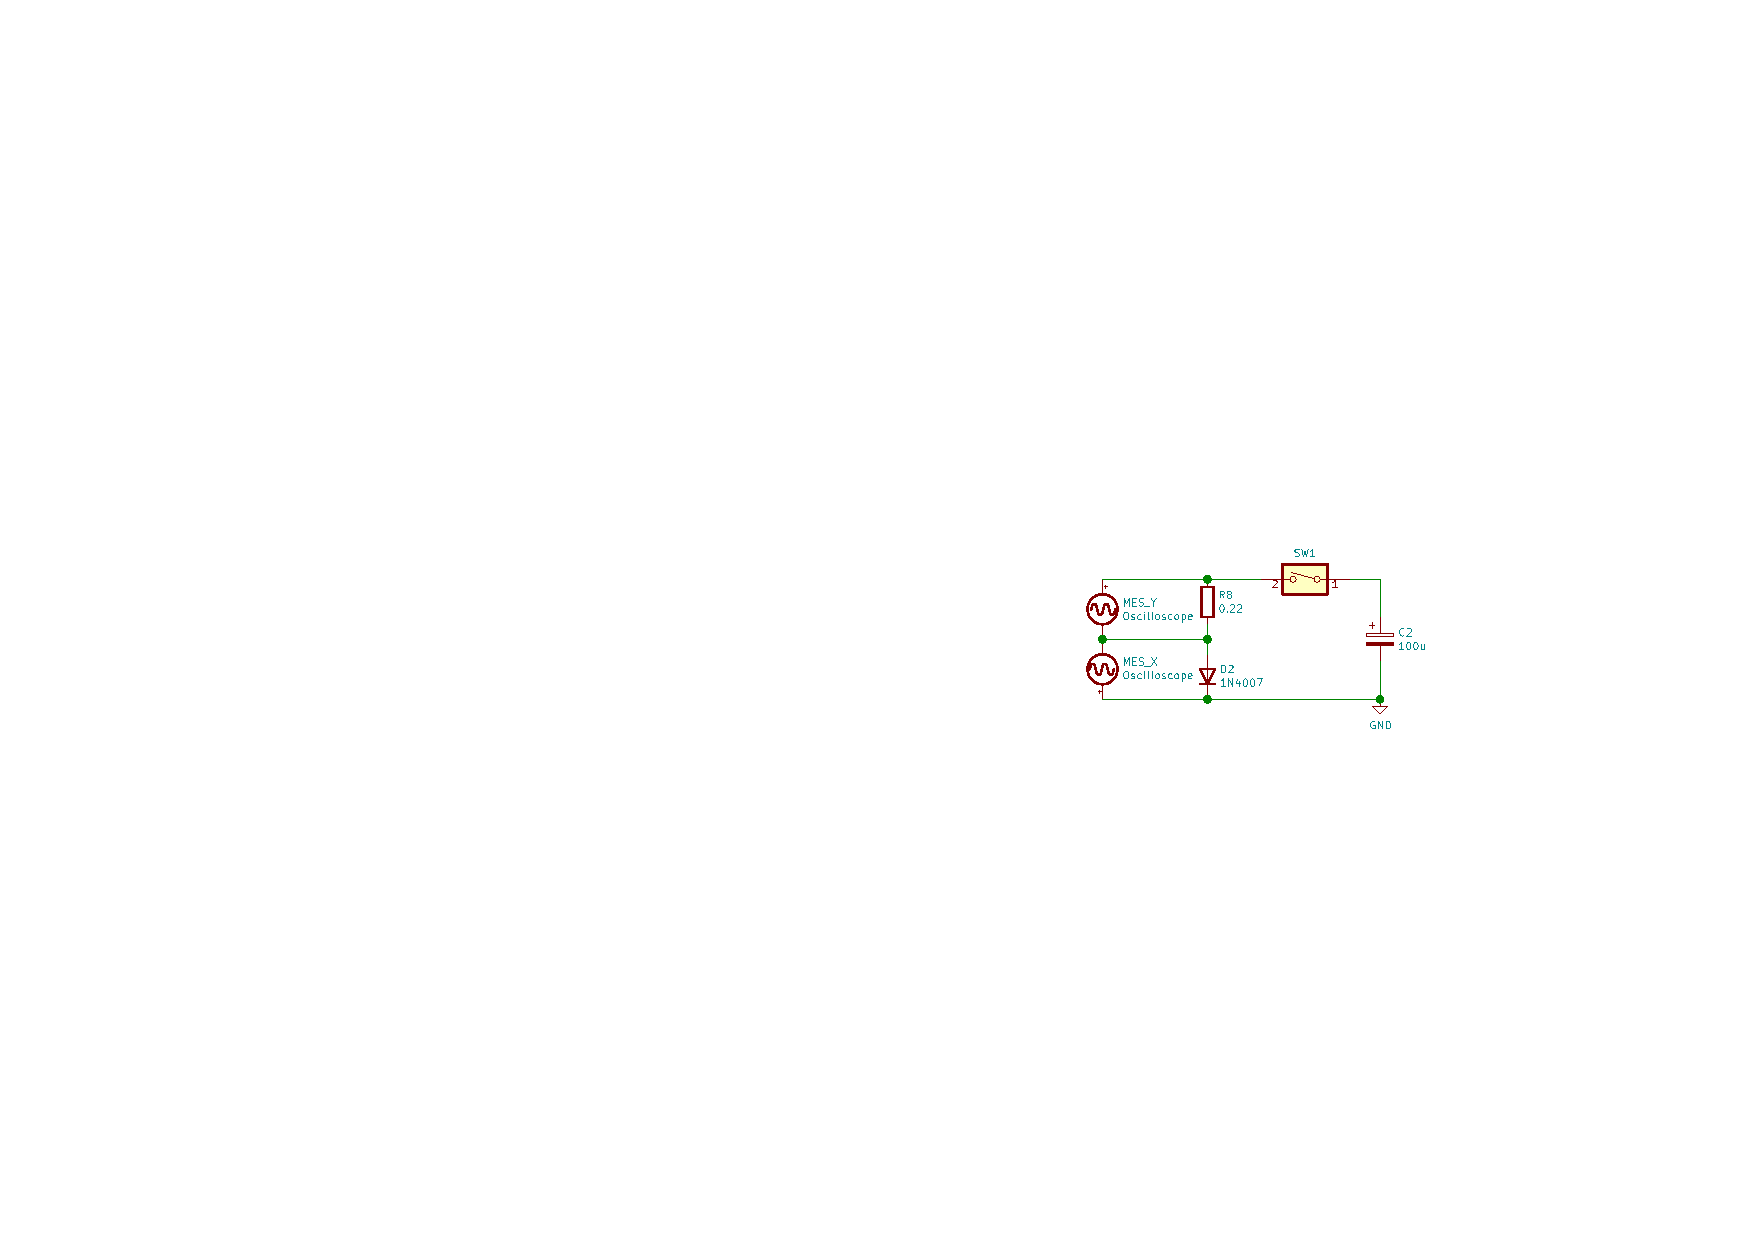
\includegraphics[scale=2.2]{./simple.pdf}
 	\caption{Versione semplice del circuito \label{sch:smpl}}
\end{figure}
\begin{figure}[!htb]
	\centering 
 		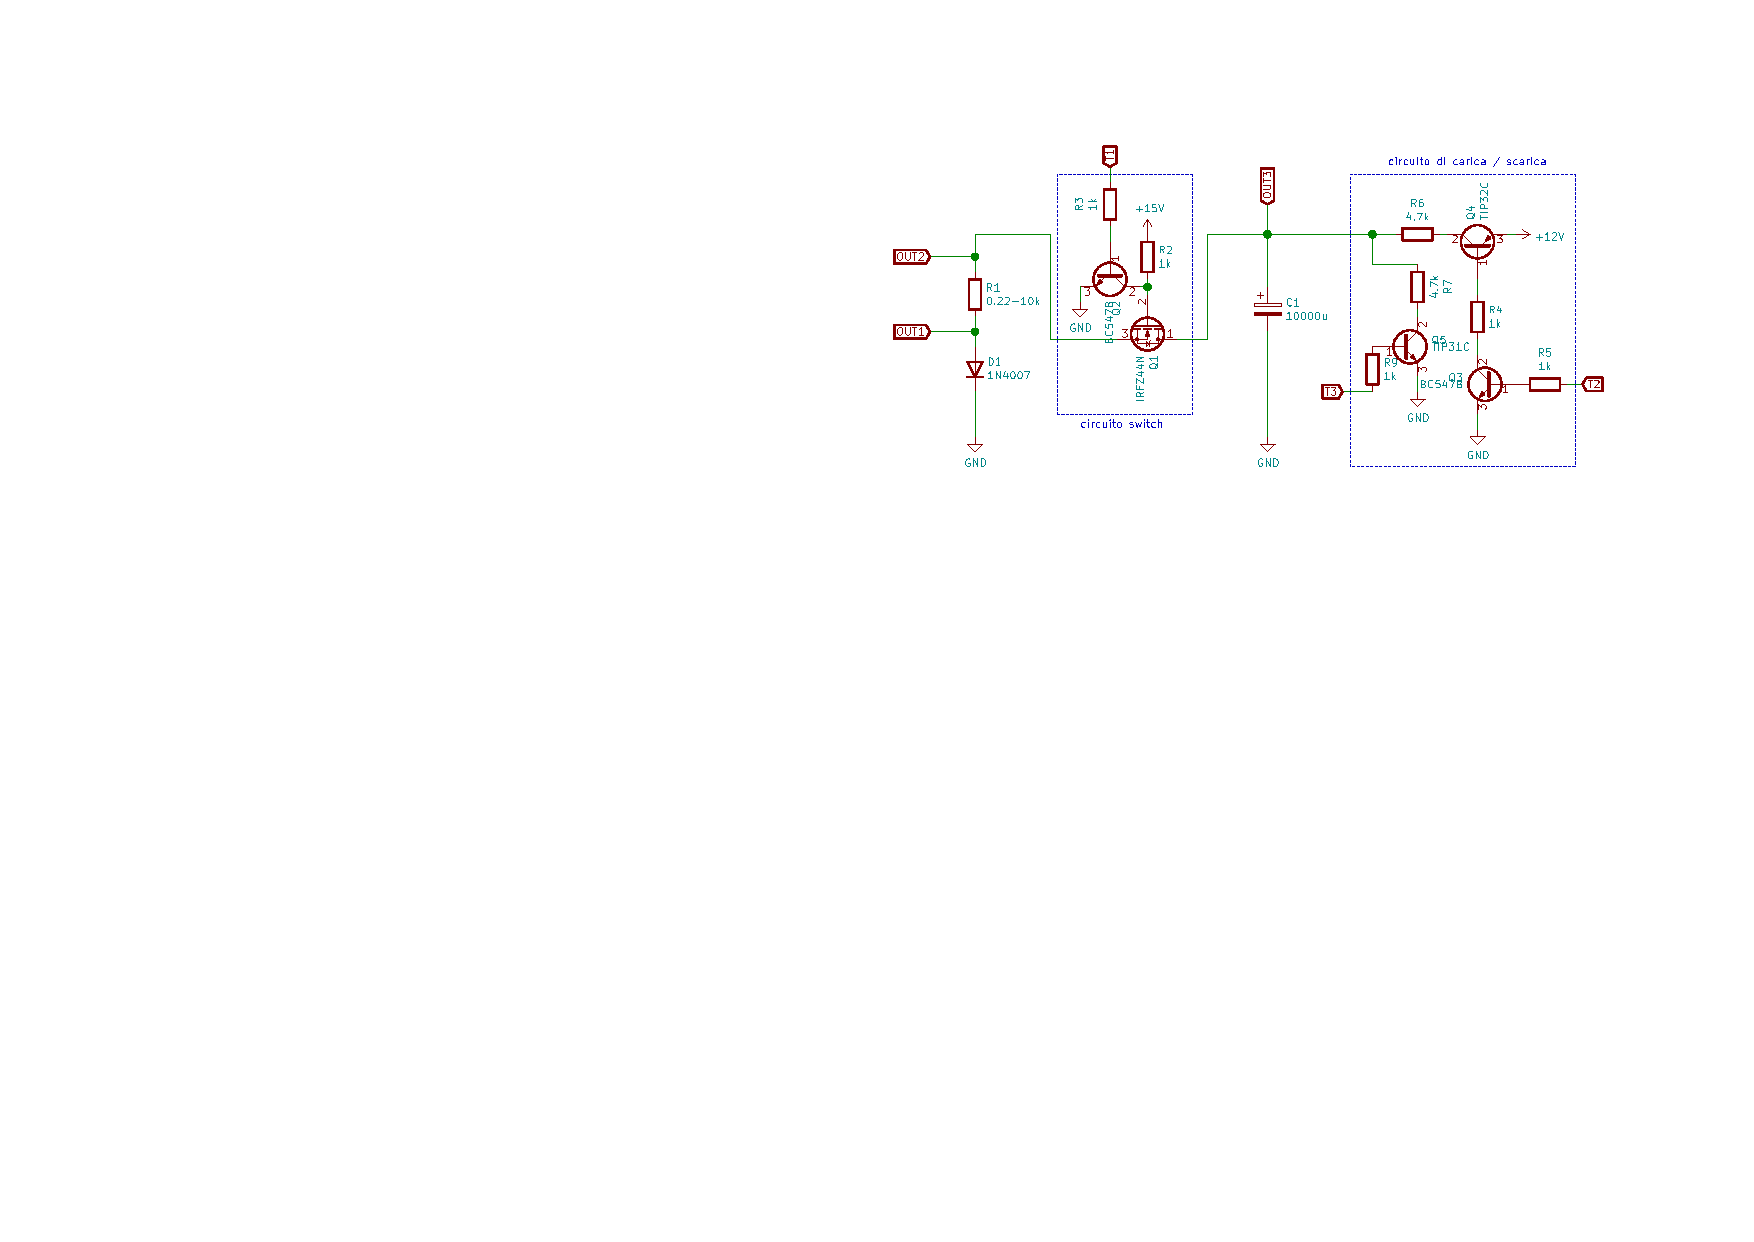
\includegraphics[scale=1.3]{./gestione.pdf}
 	\caption{Circuito globale per la gestione del diodo \label{sch:gest}}
\end{figure}
\begin{figure}[!htb]
	\centering 
 		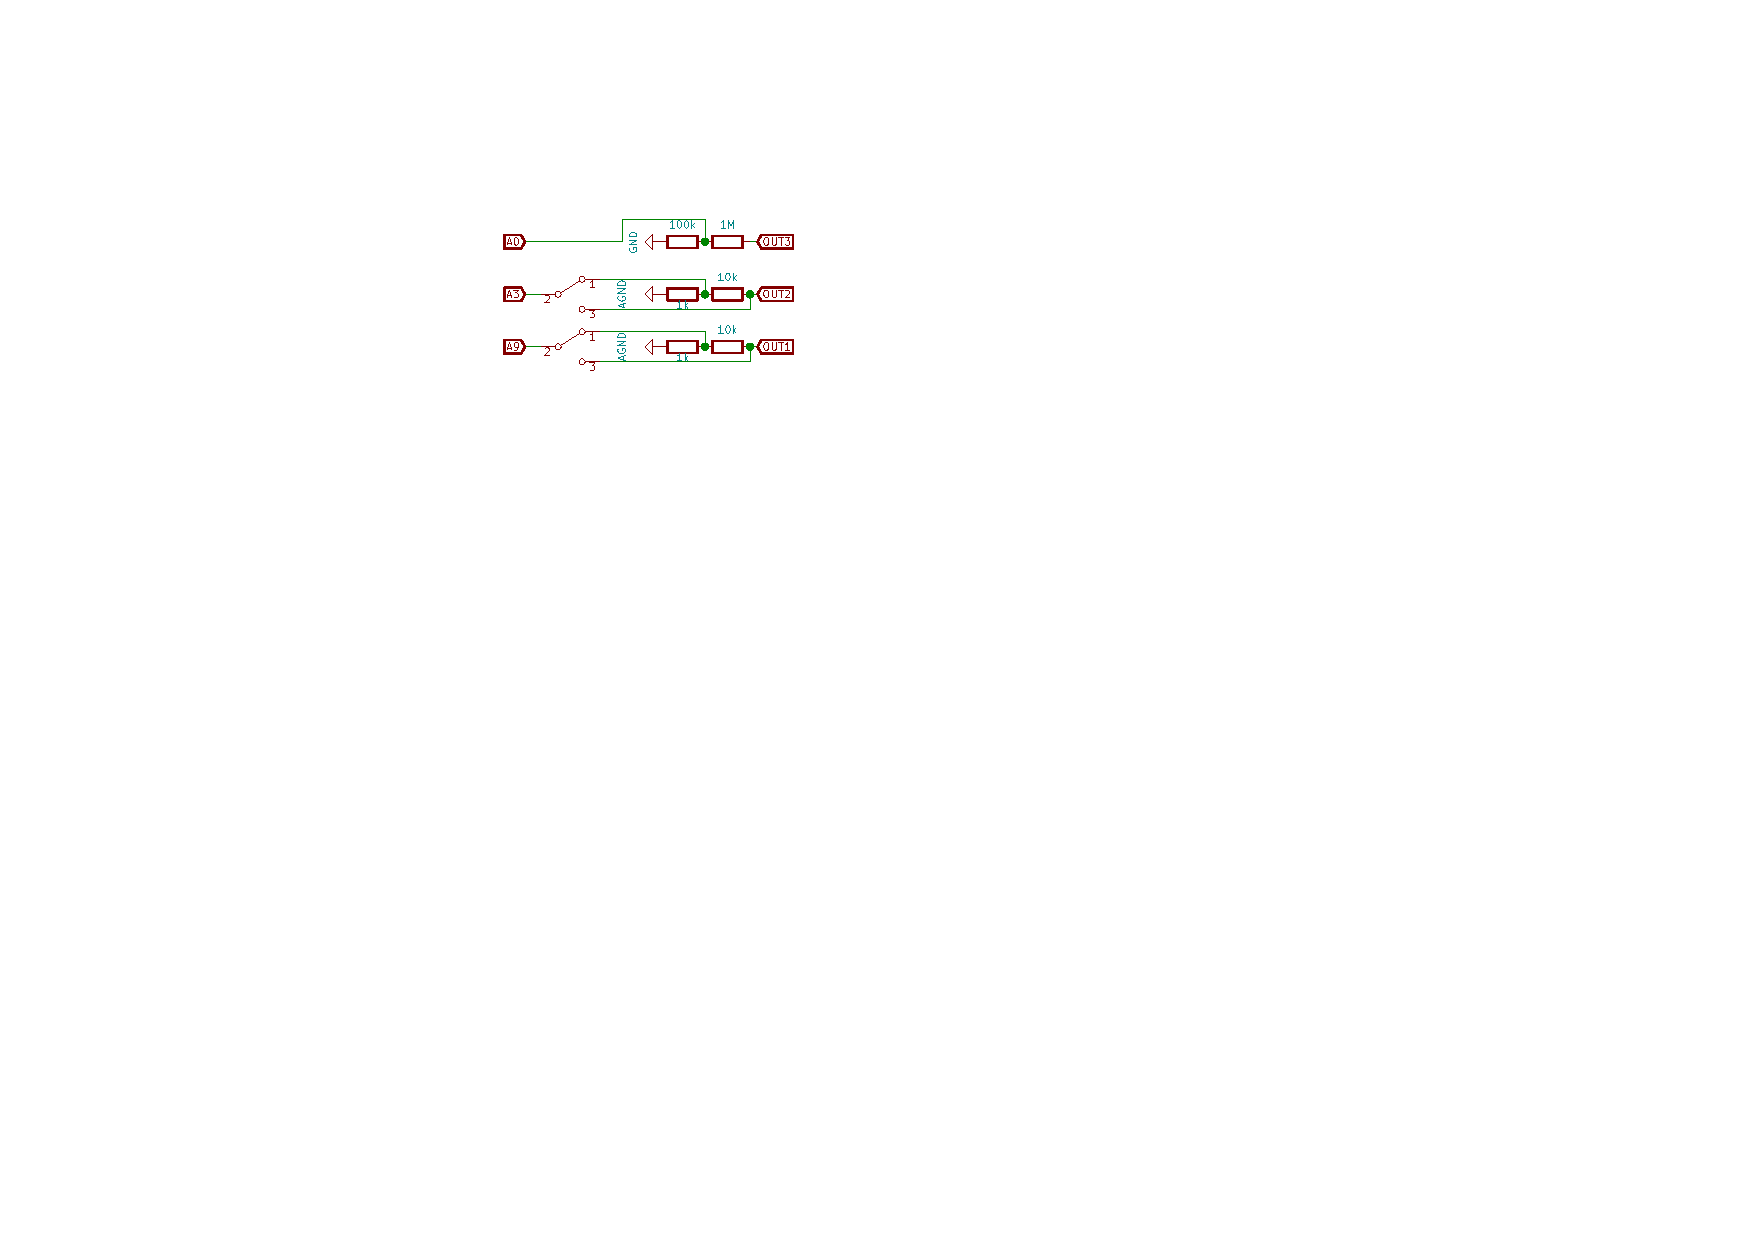
\includegraphics[scale=2.2]{./measure.pdf}
 	\caption{Schema circuitale del sistema di lettura (\texttt{Teensy})
	\label{sch:rdng}}
\end{figure}
Come ultima cautela preliminare, per minimizzare le influenze esterne sulla
misura della componente resistiva del diodo, si sono misurate le resistenze dei
collegamenti del circuito, in quanto i cavi reali e gli ingressi del diodo
possono avere resistenze non trascurabili rispetto a quella opposta dal diodo
in regime di conduzione, nell'ordine di qualche ohm.

Tramite il semplice circuito con interruttore in Figura \ref{sch:smpl} riusciamo
a ricostruire sperimentalmente la curva caratteristica V-$I$ del diodo: si
lascia scaricare repentinamente il condensatore sulla serie diodo-resistenza
chiudendo l'interruttore, dunque dai canali di un oscilloscopio si misura la
curva risultante.

Vista la stabilità poco attendibile del circuito con interruttore azionato
manualmente si è costruito una seconda versione del circuito (Fig.
\ref{sch:gest}), in cui figura un sottocircuito di switch e un condensatore di
capacità maggiore di un paio di ordini di grandezza. Infine si aggiunge la
maglia a destra del condensatore, impiegata per caricare (e scaricare) quest'
ultimo a diverse tensioni, controllate grazie a \verb+Teensy+.
Si sviluppano due casi principali:

Se lasciamo caricare gradualmente il condensatore, essendo $C$ decisamente
maggiore rispetto ai condensatori precedenti si ha un tempo di carica
$\tau = RC$ abbastanza prolungato, in cui possiamo campionare contemporaneamente
tensione e corrente ai capi del diodo per correnti modeste, nel regime in cui
il diodo è "interdetto" ed oppone resistenza al flusso di carica.

Viceversa, nel regime in cui si applichi al diodo una d.d.p. ben al disopra di
$V_{\rm thr} \approx 0.6 $V, che siamo liberi di esplorare variando la tensione
di carica di C con il sottocircuito destro, il diodo idealmente lascia passare
tutta la corrente impressa sulla giunzione. Allora per caratterizzare la
risposta del diodo senza cambiarne drasticamente le caratteristiche (ad esempio
per eccessiva agitazione termica) si impiega il circuito di switch per
imprimere impulsi di alta corrente e breve durata sulla giunzione PN, di cui
misuriamo la curva caratteristica in risposta con i due ADC di \verb+Teensy+. 

Se effettivamente il diodo, oltre ad una certa soglia di d.d.p. inizia ad avere
componente resistiva sempre più pronunciata, allora riportando le nostre
previsioni in carta semilogaritmica ci si aspetterebbe di trovare una retta,
entro il regime in cui è valida l'approssimazione di Shockley, ma oltre a
questo, una regione in cui la curva caratteristica della giunzione ora mostra
una dipendenza apprezzabilmente più lineare/ohmica dell'intensità di corrente
dalla $\Delta$V rispetto a prima, a cui corrisponderebbe il grafico "piatto"
di un logaritmo.  \section{Risultati e Analisi dati}
\subsection{Nota sul metodo di fit}
Per determinare i parametri ottimali e le rispettive varianze si \`e
implementato un metodo di fit basato sui minimi quadrati in \verb+Python+
mediante la funzione \emph{curve\_fit} della libreria Scipy\cite{scipy}.
\medskip
\bibliographystyle{IEEEtrandoi}
\bibliography{refs}
\end{document}
